\section{Use Cases principaux }

\begin{figure}[H]
  \caption{Diagramme UML use case}
  \centering
  \vspace*{0.5cm}
  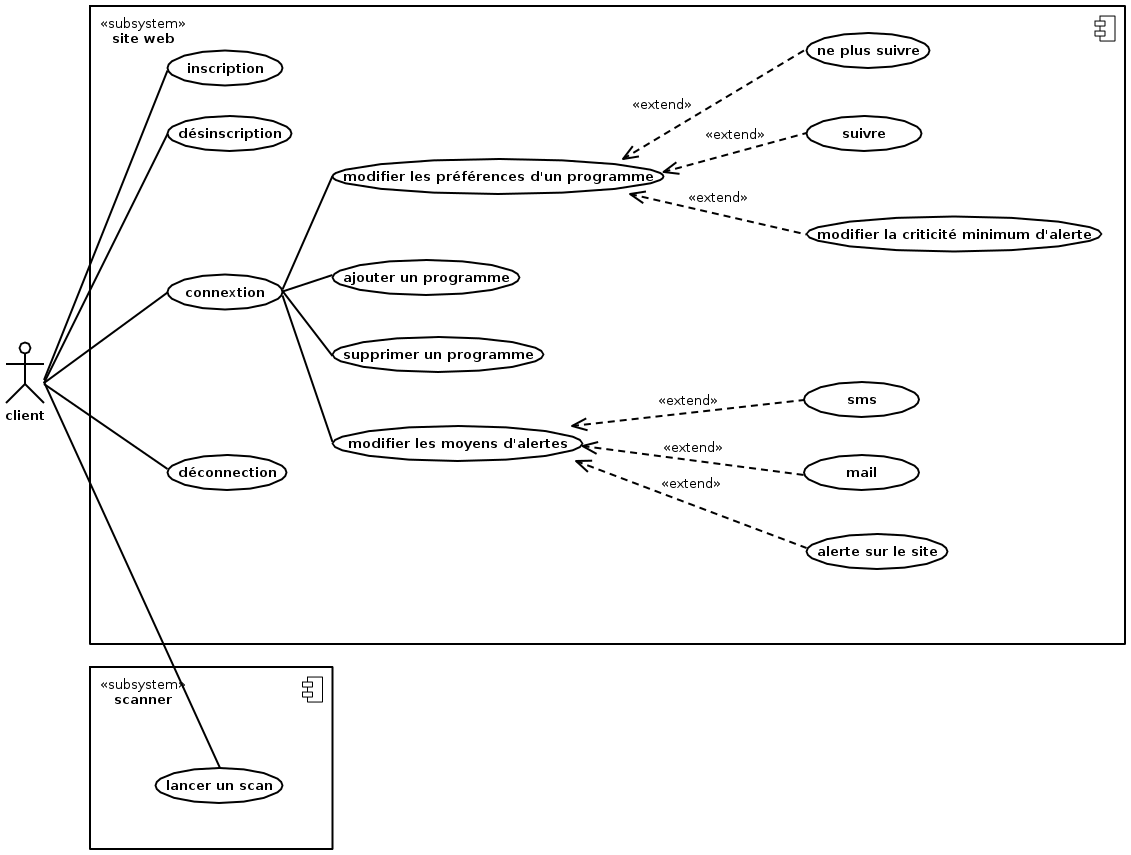
\includegraphics[width=10cm]{usecase.png}
\end{figure}

\section{Use cases détaillés}
Le client peut : s'inscrire, se désinscire, se connecter, se déconnecter, lancer le programme de scan sur sa machine.\\
Dans le cas de la connexion, l'utilisateur peut:\\
\begin{itemize}
\item Modifier les préférences d'un programme (suivre/ne plus suivre/modifier la criticité)\\
\item Ajouter un programme\\
\item Supprmer un programme\\
\item Modifier les moyens d'alertes (sms/mail/alerte sur le site\\
\end{itemize}